\documentclass[conference]{IEEEtran}
\IEEEoverridecommandlockouts
% The preceding line is only needed to identify funding in the first footnote. If that is unneeded, please comment it out.
\usepackage{cite}
\usepackage{amsmath,amssymb,amsfonts}
\usepackage{algorithmic}
\usepackage{graphicx}
\usepackage{textcomp}
\usepackage{xcolor}
\usepackage{amsmath,graphicx}
\usepackage{verbatim}
\newcommand{\para}[1]{\noindent\textbf{#1}}
\def\x{{\mathbf x}}
\def\L{{\cal L}}
\newcommand{\comments}[1]{}
\def\BibTeX{{\rm B\kern-.05em{\sc i\kern-.025em b}\kern-.08em
    T\kern-.1667em\lower.7ex\hbox{E}\kern-.125emX}}
\begin{document}

\title{Training semantic segmentation networks with temporal consistency}
%\title{Semi-supervised learning for semantic segmentation}
%{\footnotesize \textsuperscript{*}Note: Sub-titles are not captured in %Xplore and
%should not be used}
%\thanks{Identify applicable funding agency here. If none, delete this.}
%}

\author{\IEEEauthorblockN{1\textsuperscript{st} Feiyu Qin}
\IEEEauthorblockA{\textit{University of Science and Technology of China}\\
Heifei, China \\
feiyuqin@mail.ustc.edu.cn}
\and
%\IEEEauthorblockN{2\textsuperscript{nd} Lumeng Cao}
%\IEEEauthorblockA{\textit{University of Science and Technology of China}\\
%	Heifei, China \\
%	clm@mail.ustc.edu.cn}
%\and
\IEEEauthorblockN{2\textsuperscript{rd} Xuejin Chen}
\IEEEauthorblockA{\textit{University of Science and Technology of China}\\
	Heifei, China \\
	xjchen99@ustc.edu.cn}
}
\maketitle
\begin{abstract}
Semantic segmentation is a fundamental task in indoor scene understanding. 
Most previous supervised approaches rely on densely annotated image datasets. 
Due to the limited amount of images with segmentation labels, the performance and robustness of existing networks is greatly limited.
In this work, we exploit spatical and temporal correlation in video frames to improve the performance of segmentation networks. 
Two effective semi-supervised learning strategies are proposed to propagate the information from a few labeled frames to adjacent video frames. 
First, we augment training data for supervised semantic segmentation networks by generating pseudo ground-truth for neighboring frames from a labeled frame using filtered homography transformation.
Second, we introduce a self-supervised loss function to ensure temporal consistency between the segmentation results of adjacent frames. 
The experimental results show that our proposed method outperforms state-of-the-art techniques for semantic segmentation on NYU-Depth V2 dataset.

\end{abstract}
\begin{IEEEkeywords}
	Indoor scene, semantic segmentation, temporal consistency, label propagetion 
\end{IEEEkeywords}
\section{Introduction}
\label{sec:intro}
%Nowadays, advent of consumer friendly and affordable depth-cameras such as Kinect are commercially employed in many applications such as robotics and virtual reality.
%Understanding and interpreting raw data provided by depth-cameras has drawn many attentions of researchers.
%

\begin{comment}
\begin{figure}[t]
	\includegraphics[scale=0.65]{figure/Consist.png}
	\vspace*{-0.6cm} 
	\caption{An illustration of jumping problem in video semantic segmentation. The predicted results of adjacent frames by different methods are shown. Our method generates more temporally consistent results, especially in the highlighted regions.}
	\label{fig:Consist}
	\vspace*{-0.35cm}
\end{figure}
}
\end{comment}

Semantic segmentation is a fundamental part of scene understanding.
%
For indoor scenes, the cluttered backgrounds, large variety of scenes, object occlusions and various illumination pose a series of challenges for accurate semantic segmentation.
%
In recent years, a great deal of studies have been conducted for indoor scene semantic segmentation, and they can be mainly divided into three groups: semantic segmentation of a single RGB image, semantic segmentation of RGBD images, and multi-task learning methods.
%



\noindent \textbf{Semantic Segmentation of a Single Image.}
%
Fully convolutional network (FCN)~\cite{Long2015} is a pioneering work for pixel-wise segmentation. It first converts existing convolutional neural networks (CNN) constructed from classification to semantic segmentation.
%
To overcome the limitations of FCN that the network limited by a fixed-size receptive field, Noh \emph{et al.} \cite{Noh2015} proposed a novel deconvolution algorithm to segment finer object structures.
%
Bayesian SegNet~\cite{Kendall2015} performs visual scene understanding with a measure of model uncertainty to produce a probabilistic segmentation result.
%
To capture semantic correlations between neighboring patches and exploit patch-patch contextual information, Lin \emph{et al.}~\cite{Lin2016} formulated conditional random fields (CRFs) with CNN-based pairwise potential function. 
%
For generating fine prediction, a multi-path refinement network is proposed to effectively exploit multi-level features and refine the prediction step by step~\cite{Lin2017}.
%

\begin{figure*}[htbp]
%	\vspace{-0.6cm}
	\setlength{\abovecaptionskip}{0pt} 
	\setlength{\belowcaptionskip}{10pt}
	\centering
	\centering
	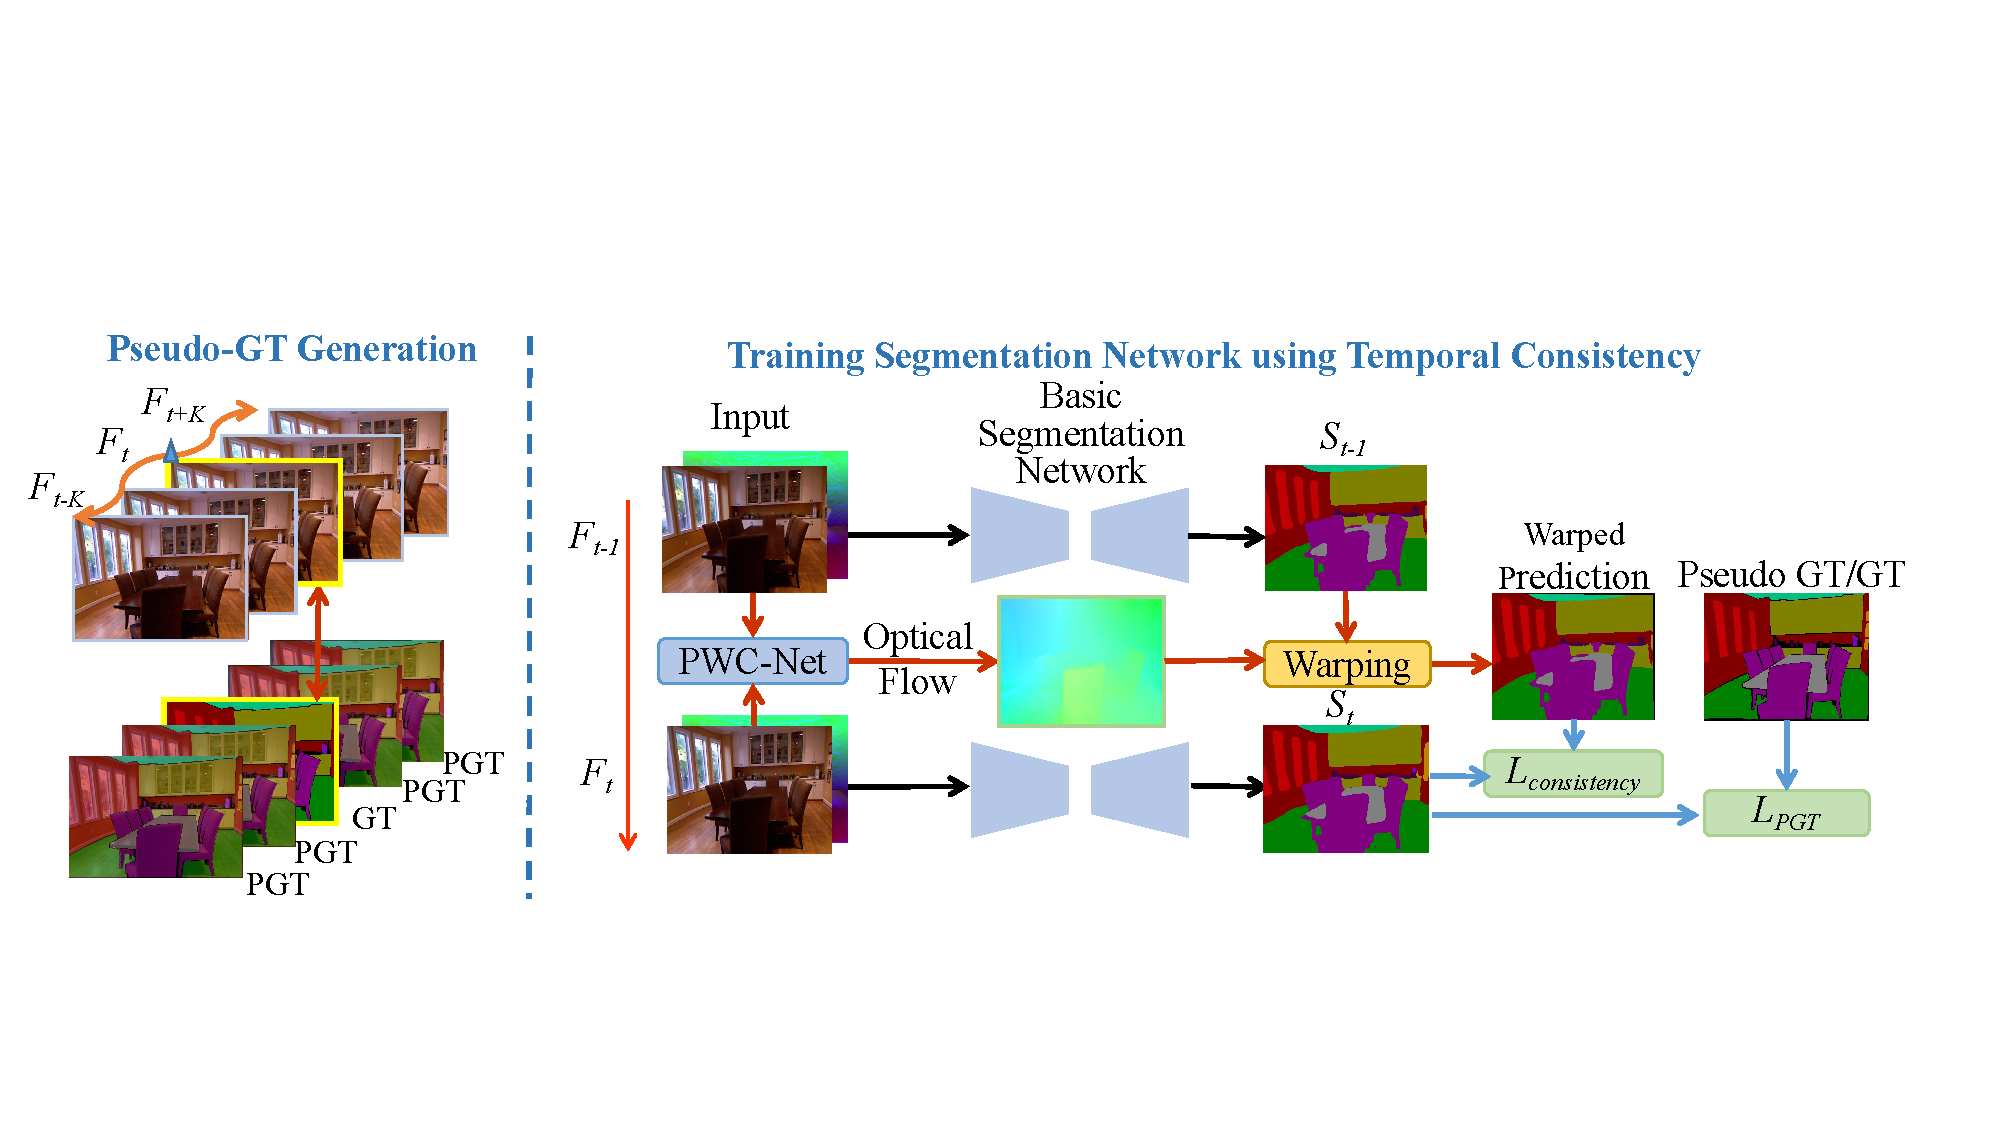
\includegraphics[scale=0.56]{figure/Pipeline.pdf}
%	\vspace*{-0.8cm} 
	\caption{The diagram of our proposed method. Left: we propagate the ground truth from a labeled frame to its adjacent frames by image warping. Right: the flowchart of our training strategy using temporal consistency. 
	It mainly consists of three steps: 1) The current frame $F_t$ passes through a basic semantic segmentation network to generate the prediction $S_{t}$ 2) Warping the prediction $S_{t-1}$ of previous frame $F_{t-1}$ depends on optical flow generated from PWC-Net \cite{Sun2018} 3) Warped prediction of $F_{t-1}$ and generated PGT joint action on the network by $L_{Consistency}$ and $L_{PGT}$ respectively.
		}
	\label{fig:Pipeline}
	\vspace*{-0.2cm}
\end{figure*}
 

\noindent \textbf{Semantic Segmentation of RGB-Depth Images.}
%
With the popularity of affordable depth-cameras, many techniques have been proposed for semantic segmentation of RGBD images.
%
Gupta \emph{et al.} \cite{Gupta2014} extracted features from RGB and depth data and integrated them for object detection and segmentation.
%
A novel long short-term memorized context fusion (LSTM-CF) model is proposed \cite{Li2016} to fuse contextual information from multiple sources such as RGB images and depth data.
% 
Cheng \emph{et al.} \cite{Cheng2017} rethink the relationship between RGB images and depth, and propose a locality-sensitive deconvolution network to refine object boundaries of segmentation result as well as a gated fusion layer to combine features of two modes.
%
Park \emph{et al.} \cite{Park2017} propose a multi-modal feature fusion block for fusing the multi-level RGB-D features and integrate these blocks into RefineNet.


 
\noindent \textbf{Multi-task Learning.} 
%
While semantic segmentation, depth estimation, and other tasks for indoor scene understanding share features, especially at shallow layers, many techniques have been proposed to train networks for multiple tasks in order to complement each other.
%
Eigen and Fergus \cite{Eigen2015} address three different tasks including depth prediction, surface normal estimation, and semantic labeling using a single multi-scale convolutional network. 
%
Prediction-and-distillationn network (PAD-Net)\cite{Xu2018} predicts a set of intermediate tasks including depth, surface normal, semantic and contour estimations, and then uses the predictions from these tasks as multi-modal distillation modules' inputs for final tasks.  
%
A novel joint Task-Recursive Learning (TRL) \cite{Zhang2018} framework for semantic segmentation and depth estimation is proposed by Zhang \emph{et al}. 
%
In TRL, two tasks are alternately processed in the decoder to improve each other.
% 
Jiao \emph{et al.} \cite{Jiao2018} present an attention-driven loss for network supervision and a synergy network to learn the information sharing strategies. 
%
%By combining two tasks as well as proposed attention-driven loss, the performance of two tasks are mutually improved.
%
Although the multi-task learning methods improve the segmentation results, they require a lot of supplementary information or even dense-annotated data for other tasks.

Above approaches provide a lot of novel ideas to improve the segmentation results. However, the performance and robustness of these methods is greatly suppressed by limited densely annotated training data.
%
Obtaining a large amount of annotated semantic labels for images is expensive and time-consuming.
%
In contrast, it is economical to capture videos, and the temporal correlation between adjacent frames naturally provides more information and constraints for the semantic labels. 
%
Therefore, we propose to improve existing networks for semantic segmentation by exploiting the temporal correlation between video frames in two aspects.
%In order to take full use of a large quantity of non-annotated data, in this paper, we propose two simple but effective approaches. 

First, instead of computing loss for each annotated image individually, we train a semantic segmentation network with a self-supervised loss function to ensure the temporal consistency between adjacent frames in video sequences.
%
Second, with only a few labeled video frames, we propagate these labels to its neighboring frames with geometric transformations and generate a large number of new frames with pseudo ground truth (PGT) for network training. 
Compared to common data augmentation operations, it significantly increases the diversity of training data.
%
Many image alignment methods could be used to build correspondence of two images for label propagetion.
%
The correspondence problem between two adjacent frames in a video is often formulated as optical flow estimation. 
%
However, due to optical flow eatimation depends on the low-level features of the image to find dense correspondence, it is often inaccurate and computationally expensive.
%
Hence, in our work, the method of parametric model is selected for label propagetion.
%
The commonly used parameterized model methods are rigid body transforms and homography transformation.
%
Because there are obvious holes in the depth data collected by Kinect, and the data set does not provide the corresponding camera external parameters,
%
we refer to homography transformation for label propagation.

With above two semi-supervised training strategies, our approach improves the results of fully supervised baseline method and achieves state-of-the-art performance on semantic segmentation for indoor scenes. 
%
The rest of this paper is organized as follows.
% 
Our methodology will be introduced firstly.
%
Then, we will report the extensive experimental results as well as analyses. 
%
Finally we will draw a conclusion.

\section{Methodology}
\label{sec:metho}
In this section, we begin by formulating the problem. 
%
And then we put forward our main methods.
%
Fig.~\ref{fig:Pipeline} shows the diagram of our proposed method.
%
First, propageting the labels from the labeled frames to their adjacent frames to generate pseudo ground truth.
Then we train a segmentation network with both the manually labeled frames and frames with pseudo labels, as well as a self-supervised loss function to ensure the temporal consistency between adjacent frames.
\begin{comment}
In a set of video sequences of which only a few frames are manually labeled with pixel-wise semantic labels, we first propagate the labels from the labeled frames to their adjacent frames to generate pseudo ground truth. 
Then we train a segmentation network with both the manually labeled frames and frames with pseudo labels, as well as a loss function to ensure the temporal consistency between adjacent frames.
\end{comment}
\subsection{Problem formulation}
In a set of video sequences $X := (x_1,...,x_m,x_{m+1},...,x_n)$ of which only a few frames $X_M := (x_1,...,x_m)$ are manually labeled with pixel-wise semantic labels $Y_M := (y_1,...,y_m)$. 
%
The remaining frames $X_U := (x_{m+1},...,x_n)$ are unlabeled.
%
The goal in our semi-supervised learning is to use both labeled frames and part of unlabeled frames to train a semantic segmentation network that provides the prediction of unseen frames.

\subsection{Pseudo Ground Truth Generation}
%
In a video sequence of which one frame $F_t$ is manually annotated with pixel-wise semantic labels $G_t$, we propagate these labels to its adjacent $2K$ frames $\mathcal{F}=\{F_{t-K},\ldots, F_{t+K}\}$ via two steps.
%
First, for each frame $F_k$ in $\mathcal{F}$, a homography matrix $\mathbf{H}_{tk}$ is first computed by looking for matched SIFT keypoints with RANSAC verification.
%
In order to avoid large distortion or content changes, we only keep the video frames whose transformation matrix to the reference frame $F_t$
% 
\begin{equation}
\centering
\begin{aligned}
\mathbf{H}_{tk}
=
\left[
\begin{array}{ccc}
h_{00} & h_{01} & h_{02}\\
h_{10} & h_{11} & h_{12}\\
h_{20} & h_{21} & 1\\
\end{array}
\right] \\
s.t. \hspace{0.2cm}0.95<\max{\left\{\left|h_{00}\right|,\left|h_{01}\right|,\left|h_{10}\right|,\left|h_{11}\right|\right\}}&<1.05,\\
\max{\left\{\left|h_{02}\right|,\left|h_{12}\right|,\left|h_{20}\right|,\left|h_{21}\right|\right\}}&<15.\\
\end{aligned}
\end{equation}


Fig.~\ref{fig:PGT} shows an example of the generated pseudo ground truth labels from a reference frame $F_t$. 
It can be seen that most of the semantic labels are well propagated and can be used as extra data for network training. 
% 
However, there are still some noisy labels in the propagated PGT, especially at the object boundary regions. 
%
Therefore, we add a manual filtering process to remove the frames where there are obvious visual artifacts in the generated pseudo labels.

A toy example showing the results of label propagetion by our method, rigid body transformation and flow estimation is shown in Fig.~\ref{fig:PGT_Com}.
%
Compared to other PGT generated methods, our approach keeps the boundary of PGT better.

\begin{figure}[t]
	\centering
	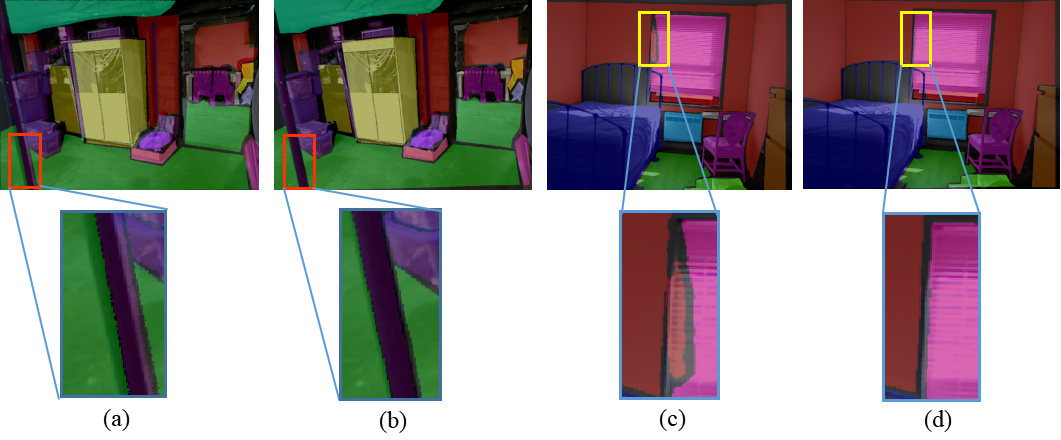
\includegraphics[width=\columnwidth]{figure/PGT_compared.png}
	%	\vspace*{-0.6cm} 
	\caption{Comparison of different methods of annotation propagetion. (a) PGT generated by rigid body transformation. The camera external parameters is evaluated by Bundler and the depth is filled using NYU-v2 official code. (b)(d) PGT of our method. (c) PGT generated by optical flow using PWC-Net\cite{Sun2018}.}
	\label{fig:PGT_Com}
	%	\vspace*{-0.35cm} 
\end{figure}

%\noindent\textbf{Training Segmentation Network using Temporal Consistency.}
\subsection{Training Segmentation Network using Temporal Consistency}
%
As Fig.~\ref{fig:Pipeline} shows, we train a semantic segmentation network using two adjacent frames in a video instead of using a single labeled frame.  
% 
First, two adjacent frames $F_{t-1}$ and $F_t$ are passed through a basic segmentation network to predict semantic labels $S_{t-1}$ and $S_{t}$.
%
The basic segmentation network could be any existing network for semantic segmentation. 
We use RDFNet\cite{Park2017}, which is a high-precision network for semantic segmentation of a RGBD image.
% The input of RDFNet is a RGBD image. 
%The depthmap is encoded into a 3D image called HHA \cite{Gupta2014} which encodes {\bf H}eight above ground and {\bf H}orizontal disparity in addition to the {\bf A}ngle with gravity for each pixel .
%Four multi-model feature fusions (MMF) are used to fully exploit multi-level HHA and RGB images' features.
% And then four RefineNet blocks are applied to refine the output of MMF gradually.
% More details of RDFNet could be found in \cite{Park2017}. 



Second, the predicted semantic score map $S_{t-1}$ for frame $F_{t-1}$ is warped to $\hat{S}_{t}$ according to the optical flow $O_{t-1,t}$ between $F_t$ and $F_{t-1}$, which is estimated using an efficient and accurate model PWC-Net~\cite{Sun2018} from two frames. 
We implement a bilinear interpolation for $40$ dimensional score vector of each pixel in $S_{t-1}$, where 40 is the total number of object classes in the dataset. 
\begin{equation}
\centering
\hat{S}_{t}=Warp(S_{t-1},O_{t-1,t}).
\end{equation}
%
An argmax layer is then added on the warped score map ${\hat{S}_{t}}$ to generate the warped semantic prediction $W_{t}$.
\begin{comment}
\begin{equation}
\centering
W_{t}=\arg \max \hat{S}_{t-1}.
\end{equation}
\end{comment}


Finally, the warped prediction $W_{t}$ acts as a self supervised item to constrain the consistency of prediction results between neighboring image frames.
%
Meanwhile, the PGT of current frame $F_t$ acts as another supervisory item to guarantee that the prediction results are as accurate as possible.
Combining these two items, our loss function is defined as
\begin{equation}
\centering
\begin{aligned}
L_{seg}= \lambda L_{Consistency} +(1-\lambda)L_{PGT},
\end{aligned}
\end{equation}
%
where, ${L_{PGT}}$ and ${L_{Consistency}}$ are cross-entropy loss, defined as
\begin{equation}
{
\vspace*{-0.6cm} 
\centering     
\begin{aligned} 
L_{Consistency} &= -\sum_{i=0} l(\mathbf{w}_i,\mathbf{y}_i),\\
L_{PGT} = -&\sum_{i=0} l(\mathbf{p}_i,\mathbf{y}_i), \\
l(\mathbf{p}_i,\mathbf{y}_i) = -&\sum_{k=0}^c \,\mathbf{p}_{ik}\log{\mathbf{y}_{ik}}\;,\; \mathbf{y}_{i} = f(x_{i}),\\
\end{aligned}
}
\end{equation}
%
where ${x_i}$ and ${\mathbf{y}_i}$ are a pixel of an input frame and the corresponding predicted output of the semantic segmentation model respectively. 
%
$\mathbf{y}_i$ is a $c$ dimensional probability vector for each pixel.
${c}=40$ is number of categories.
%
${\mathbf{p}_i}$ and ${\mathbf{w}_i}$ are an one-hot vector for each pixel of the pseudo ground truth or ground truth label, and warped prediction $W_{t}$ from previous frame, respectively. 
%
${l(\cdot)}$ is the softmax loss of one pixel, and ${f(\cdot)}$ is our basic segmentation network. 
%
By these two losses, we can constrain the accuracy and temporal consistency of the network prediction simultaneously.

\section{EXPERIMENTS AND EVALUATION}
\label{sec:exper}

\begin{figure}[t]
	\centering
	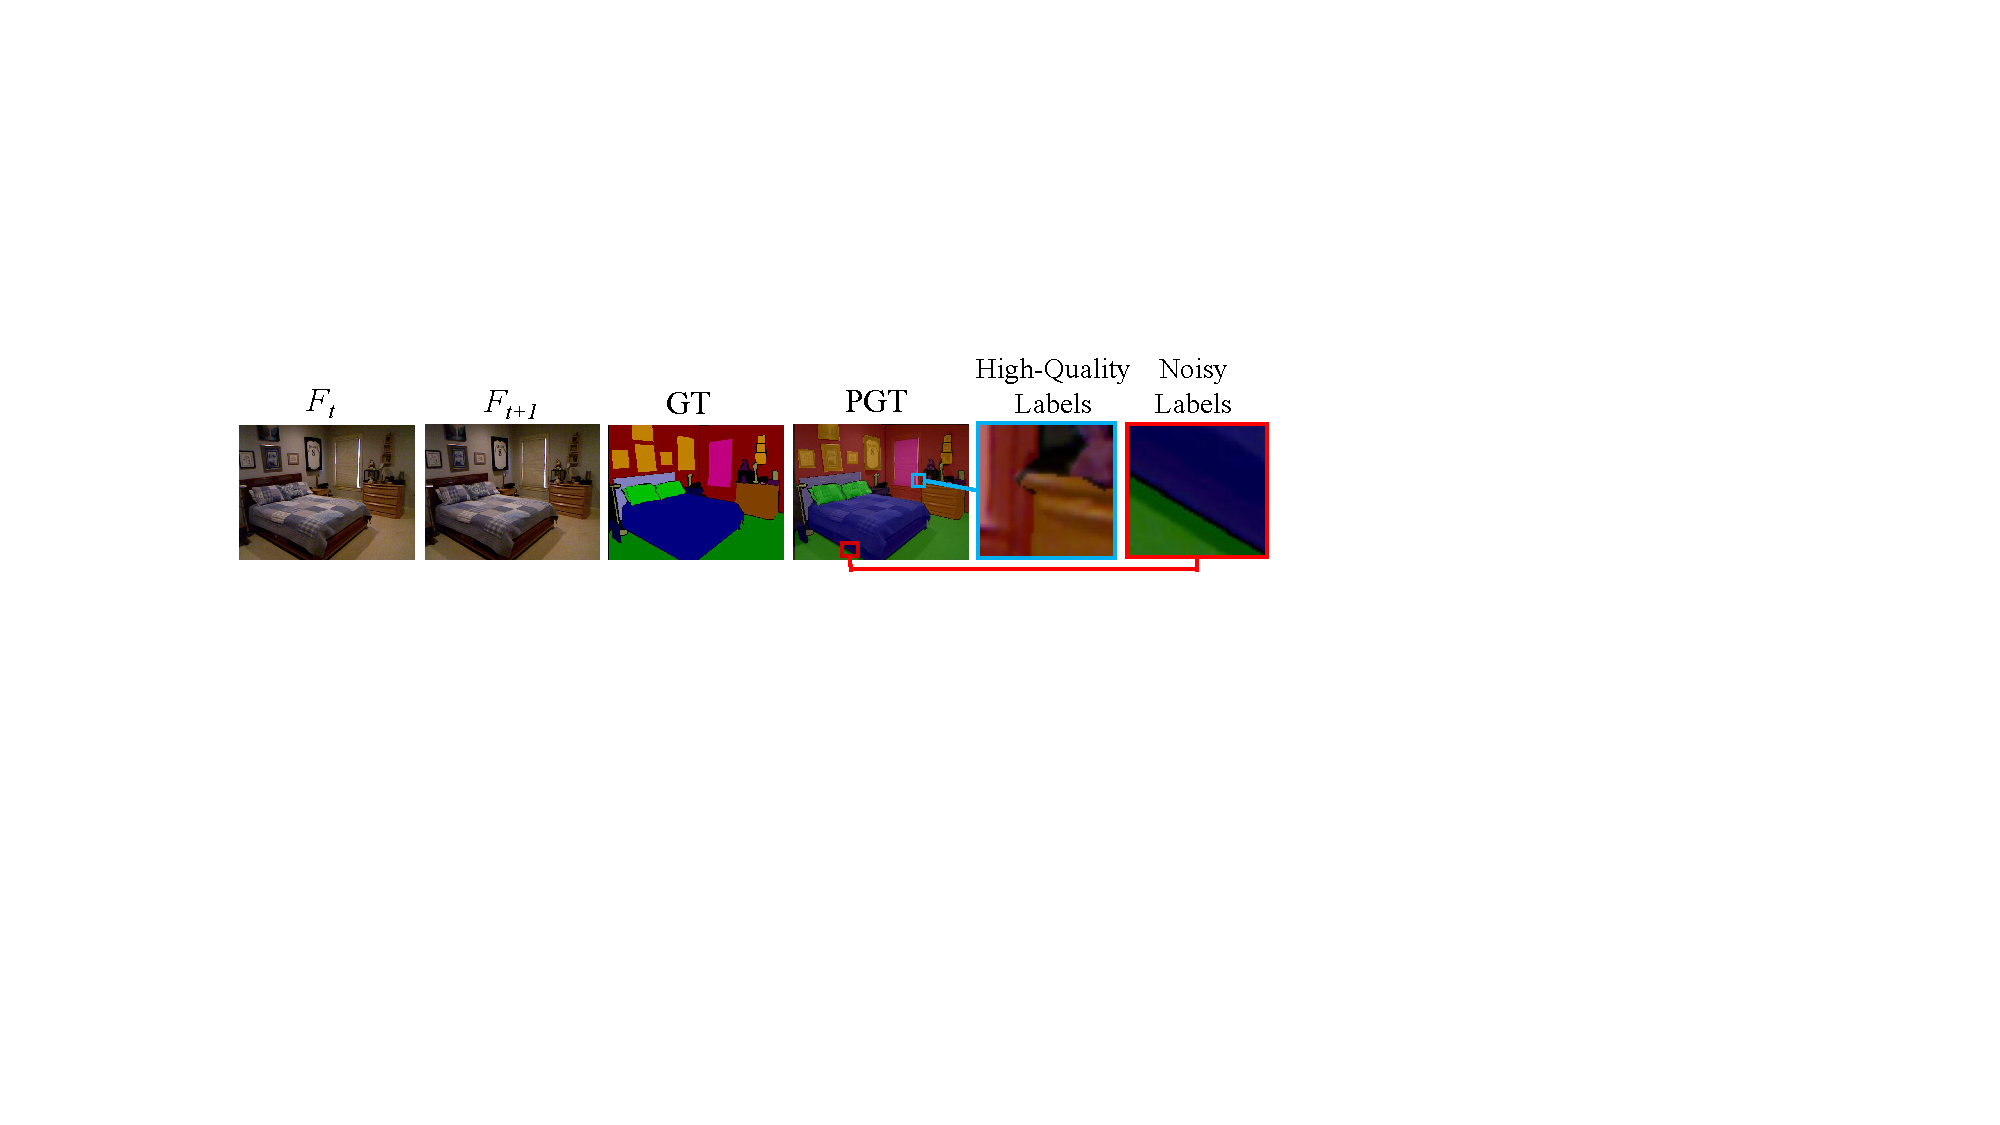
\includegraphics[width=\columnwidth]{figure/PGT.pdf}
	%	\vspace*{-0.6cm} 
	\caption{Propagated pseudo ground truth from a reference frame $F_t$ to $F_{t+1}$. Most of the pseudo labels are reliable, while there are some noisy around object boundaries.}
	\label{fig:PGT}
	%	\vspace*{-0.35cm} 
\end{figure}


In order to evaluate the proposed method for indoor scene segmentation, we conduct experiments on a publicly available benchmark dataset (NYUD-v2) and show the superiority of our method.
%, which contains 273 video sequences of RGBD data.  

\begin{figure}[!th]
	\centering
	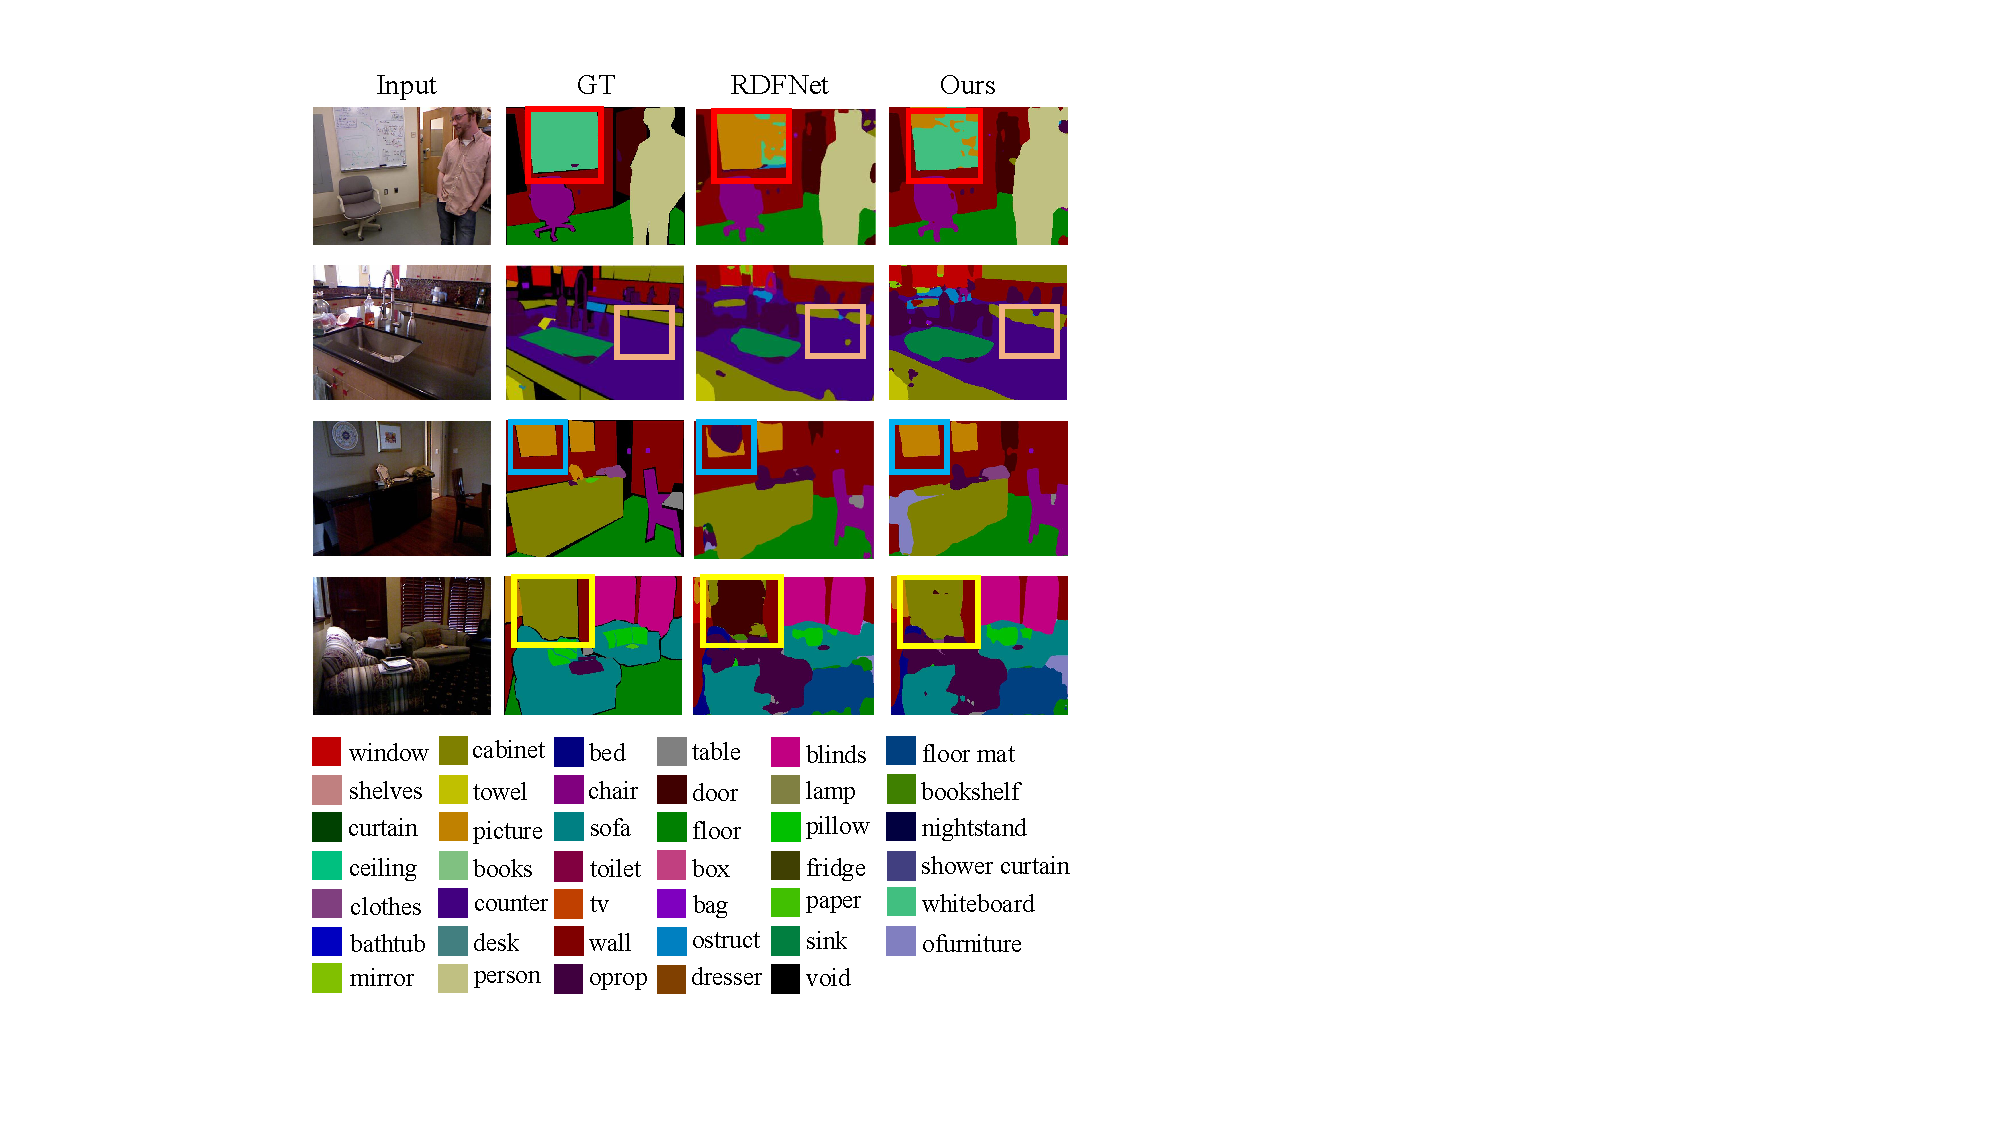
\includegraphics[width=\columnwidth]{figure/Result.pdf}
	\caption{Qualitative results on the NYUD-v2 dataset. In each row, we show the input image, the ground truth of semantic segmentation, the result of RDFNet, and the result of our method, from left to right, respectively. Our method predicts more accurate segmentation results, especially at hhe highlighted regions.}
	\label{fig:VisResult}
	\vspace*{-0.3cm}
\end{figure}

\noindent\textbf{Dataset.}  
The NYUD-v2 dataset contains in total 464 diverse indoor scenes and the corresponding video sequences. 
%
For the task of semantic segmentation, 1449 images are manually annotated, among which 795 images are used for training and the remaining 654 images for testing.
%
In our experiment, we map the semantic labels into 40 categories, similar as \cite{Gupta2014}.
%
From the 795 manually labeled images for training, we propagated these GT labels to 14344 unlabeled frames, and filtered out 5897 frames by homography matrices, and filtered out 821 frames by manual check. 
We finally obtained 7626 frames with pseudo ground truth. 
%
Comparing with dense image annotation, filtering PGT for 273 videos took about 8 hours for a graduate student.
%
Although the generated pseudo labels still have a certain amount of noise, the diversity of training set is greatly enriched. 



The training images, including both manually labeled images and propagated images, are augmented by random horizontal flips with a possibility of 0.5, scaling with a randomly selected ratio in $\left\{0.7,0.8,0.9,1.0,1.1,1.2,1.3\right\}$ and random cropping. 
%
All our experiments are conducted on a single Nvidia Titan X Pascal GPU, using the Caffe framework.

\noindent\textbf{Evaluation Metrics.}  
Following previous work
\cite{Eigen2015,Gupta2014,Kendall2015,Lin2016,Lin2017,Li2016,Cheng2017,Park2017,Xu2018,Zhang2018,Jiao2018}, we use three quantitative metrics to evaluate our semantic segmentation results, including pixel accuracy, mean accuracy and mean IoU. 
%%
Denote $m_{kj}$ as the number of pixels of class ${k}$ classified as class ${j}$.
%Assuming 
The number of categories is $c$, and $M_{k} = \sum_{j}m_{kj}$ is the total number of pixels belonging to class $k$. 
%
And $N = \sum_{k}M_{k}$ denotes the number of all pixels in the test set.
%
The three metrics are defined as follows:
\begin{equation}\label{eq:metric}
\begin{array}{rl}
\text{pixel accuray}: &  \frac{1}{N}\sum_{k}m_{kk}, \\
\text{mean accuracy}: &\frac{1}{c}\sum_{k}\frac{m_{kk}}{M_{k}}, \\
\text{mean IoU}: &\frac{1}{c}\sum_{k}\frac{m_{kk}}{ M_{k}+\sum_{j}m_{jk}-m_{kk}}.
\end{array}
\end{equation}

%\renewcommand{\baselinestretch}{1.0}\indent\text{---} pixel accuracy: $\sum_{k}m_{kk}/I$;\\
%\indent\text{---} mean accuracy: $\frac{1}{c}\sum_{k}m_{kk}/m_{k}$;\\
%\indent\text{---} mean IOU: $\frac{1}{c}\sum_{k}m_{kk}/(m_{k}+\sum_{j}m_{jk}-m_{kk})$ ;\\




\begin{table}[tb]
%	\vspace{-0.4cm}
	\centering
	\caption{Comparison of different methods. The three columns represent three different types of methods: semantic segmentation of a single image, semantic segmentation of RGBD images and multi-task learning methods.}
	\begin{tabular*}{8.2cm}{llccc}
		\hline
		Method & Data & Pixel & Mean  & Mean\\
		       &     & accuracy & accuray  & IoU \\
		\hline 
		B-SegNet \cite{Kendall2015} & RGB &68.0 & 45.8 & 32.4 \\
		Context \cite{Lin2016} & RGB & 70.0 & 53.6 & 40.6 \\
		RefineNet \cite{Lin2017} & RGB & 73.6 & 58.9 & 46.5\\
		\hline
		Gupta et al. \cite{Gupta2014} & RGBD & -- & 35.1 &--\\
		Eigen et al. \cite{Eigen2015} & RGBD & 65.6 & 45.1 & 34.1\\
		FCN \cite{Long2015} & RGBD & 65.4 & 46.1 & 34.0 \\
		LSTM-CF \cite{Li2016} & RGBD & --& 49.4 & -- \\
		Cheng et al.\cite{Cheng2017} & RGBD & 71.9 & 60.7 & 45.9 \\
		RDFNet \cite{Park2017} & RGBD & \bf{76.0} & 62.8 & 50.1\\	
		%\hline
		Baseline &RGBD & 75.8 & 63.0 & 50.0\\
	%	Flow-PGT & RGBD & & &\\
		Ours (+$L_{C}$) & RGBD & 75.8 & 63.3 & 50.1\\	
		Ours (+$Pr$) & RGBD & 75.5 & 63.5 & 49.8\\
		Ours(+$Hm$) & RGBD & & &\\
		Ours (+$PGT$) & RGBD & 75.9 & 63.6 & 50.2\\
		Ours (+$L_{C}$+$PGT$)& RGBD & 75.8 & \bf{63.8} & \bf{50.2}\\
		\hline
		PAD-Net \cite{Xu2018} & RGB &75.2 & 62.3 & 50.2\\
		TRL \cite{Zhang2018} & RGB &76.2 & 56.3 & 46.4\\
		Jiao et al.\cite{Jiao2018} & RGB & \emph{81.1} & 62.2 & \emph{50.9}\\
		\hline		 		
	\end{tabular*}
	\label{Tab:Results}
\end{table}



We set the RDFNet~\cite{Park2017} as our baseline. 
However, due to hardware difference, using the official code, we get results (Baseline) that is slightly different from that reported in their paper (RDFNet), as shown in Table~\ref{Tab:Results}. 
We compare different variants of our approach to demonstrate the effectiveness of each component, and the results are reported in Table~\ref{Tab:Results}. 

\para{Analysis of Temporal Consistency.} While training RDFNet with the 795 manually labeled images, and our temporal consistency constraint (+$L_C$ for short), the mean accuracy increases to $63.3\%$ from $63.0\%$, and IoU increases to $50.1\%$ from $50.0\%$. 
%
The results show that training the network with self-supervised loss function could effectively imporve the performance of fully supervised baseline method.
%
The main reason why the performance improvement is not siginificant is that the information supplement of adjacent frames is not enough.

\para{Analysis of Pseudo labels.} 
Though the pseudo labels still contain a certain amount of noises, most of them are reliable, especially inside an object region. 
%
While training the RDFNet with extra images of pseudo labels, the performance (Ours+PGT) greatly increases, especially at mean accuracy ($63.6\%$), compared with the baseline.
%
To facilitate future study, we will release our dataset with pseudo labels.
%
In addition, we investigate the effect of quality of PGT on network performance.
%
Simply limiting the range of annotation propagation, the performance of baseline method begins to decline, largely due to the poor quality of PGT.
%
But on the other hand, with the increase of the number of samples, the performance (Ours+Pr) of abtained model for each category (Mean accuracy) is improved.

\begin{table*}[h]  
	\caption{Class-wise IoU on NYUD-v2}  
	\centering
	\normalsize
	%\setlength{\tabcolsep}{1mm}{
	\begin{tabular*}{16.3cm}{l|cccccccccc}  
		\hline		
		&wall &floor &cabinet &bed &chair&sofa& table& door & window& bkshelf\\   
		\hline  
		RDF-152 & 79.7 & 87.0 & \bf{60.9} & \bf{73.4}& \bf{64.6}& \bf{65.4}& \bf{50.7}& 39.9 & 49.6& 44.9\\
		Ours & \bf{80.8} & \bf{87.9} & 60.1 & 72.1& 64.1& 64.6 & 49.2 & \bf{41.6}
		& \bf{49.8}& \bf{45.3}\\
		\hline  
		\hline 
		 & counter & blind & desk& shelf&curtain& dresser& pillow& mirror& mat&cloths\\
		\hline 
		RDF-152& \bf{67.1}& \bf{63.9}& \bf{28.6}& 14.2 & 59.7&\bf{49.0} & 49.9 & 54.3& 39.4 & 26.9 \\
		Ours  & 66.6 & 61.9 & 25.1& \bf{14.4}& \bf{59.9} & 46.2 & \bf{50.1} & \bf{55.9}& \bf{41.5}&\bf{27.4}\\
		\hline 
		\hline 
		& books& refridge& tv&paper& tower& shower& box& board&person& stand\\ 
		\hline 
		RDF-152 & \bf{35.0} & 58.9& \bf{63.8} & \bf{34.1} & 41.6 & \bf{38.5} & 11.6& 54.0& 80.0 & \bf{45.3}\\ 
		Ours& 34.7 & \bf{61.4} & 61.9& 32.9 & \bf{41.7} & 37.0 & \bf{11.9}& \bf{56.8}& \bf{82.4} & 44.5\\
		\hline 
		\hline 
		& sink& lamp&bathtub& bag& othstr& othfurn& othprop& picture& ceiling& toilet\\
		\hline
		RDF-152   & 62.1& 47.1& 57.3 & 19.1 & 30.0 & 20.6& \bf{39.0}& 61.2& \bf{69.1}& 65.7\\
		Ours & \bf{65.3}& \bf{47.2}& \bf{58.5} & \bf{19.9} & \bf{32.3} & \bf{20.8}& 38.1& \bf{61.7}& 68.9 & \bf{66.5}\\
		\hline 
		\hline
	\end{tabular*}
	\label{Tab:Results_classes}
\end{table*}

Combining both the pseudo ground truth and temporal consistency, our approach outperforms existing semantic segmentation networks, especially at mean accuracy and IoU metrics. 
%
We also compare our method with three multi-task learning techniques and our method achieves comparable performance.
%
Though Jiao \emph{et al.} achieve the best performance on pixel accuracy and IoU, they require additional dense ground-truth for depth estimation and much heavier computational cost.
%
Fig.~\ref{fig:VisResult} shows a group of segmentation results. It can be seen that our method performs well on objects such as pictures, whiteboards and so on. 
%
And compared with baseline method, there is less over-segmentation in our apprrach, such as picture on the walls (Fig.~\ref{fig:VisResult}, line 3) and cabinet in the cornor (Fig.~\ref{fig:VisResult}, line 4).
%
Class-wise mean IoU of our results compared with RDFNet\cite{Park2017} are shown in Table~\ref{Tab:Results_classes}.
%
The experimental results in Table~\ref{Tab:Results_classes} show that our method effecitively improves segmentation accuracy on most categories (24/40) by using label propageting and self-supervised loss function.
%
It's not only in categories with large planes such as wall, floor and door, but also 
in classes with small size such as bag and box. 
%
Although our method imporves the performance of small objects, the mean IoU of box and bag are still under $30\%$. 
%
The main reason is that the size of these two kinds of objects is too small and the occurrence frequency of them is very low ($<25\%$).
%


\begin{comment}
\para{Analysis of Temporal Consistency.}  
To discover the effectiveness of our proposed training policy. 
%
We conduct our experiments on generated PGT data with temporal consistency loss.
%
The quantitative and qualitative results are shown in Table~\ref{Tab:Results} and
Fig.~\ref{fig:VisResult} respectively.
%
To prove that performance improvements are not just due to PGT, we did an ablation study by removing ${PGT}$.
%
The results are shown in Table~\ref{Tab:Results} and Fig.~\ref{fig:VisResult}.
%
Compared to baseline, the mean accuracy and IOU are all been promoted.
%
Using $L_{consistency}$ and $L_{PGT}$ simultaneously, the mean accuracy is improved by 0.8\%.
%
And mean IoU is improved by 0.2\%.
%
And our method achieves the comparable performance as multi-task learning method.
}
\end{comment}


\para{Dicussion.} By involving temporal consistency, we also found that there are conflicts between manual labels of the same scene, as shown in Fig.~\ref{fig:mislabels}. 
%
Compared to other methods, Our method produces much more accurate and consistent results.
%
And the feature extracted by our model is much more robust.
%
%The mean accuracy and mean IoU are under 30\%.
%
% the ground truth proposed by NYUD-v2 data set exits some annotation errors shown in Fig.~\ref{fig:mislabels}.


\begin{figure}[!htbp]
	\setlength{\abovecaptionskip}{-0.2cm}
	\setlength{\belowcaptionskip}{-10cm}
	\centering
	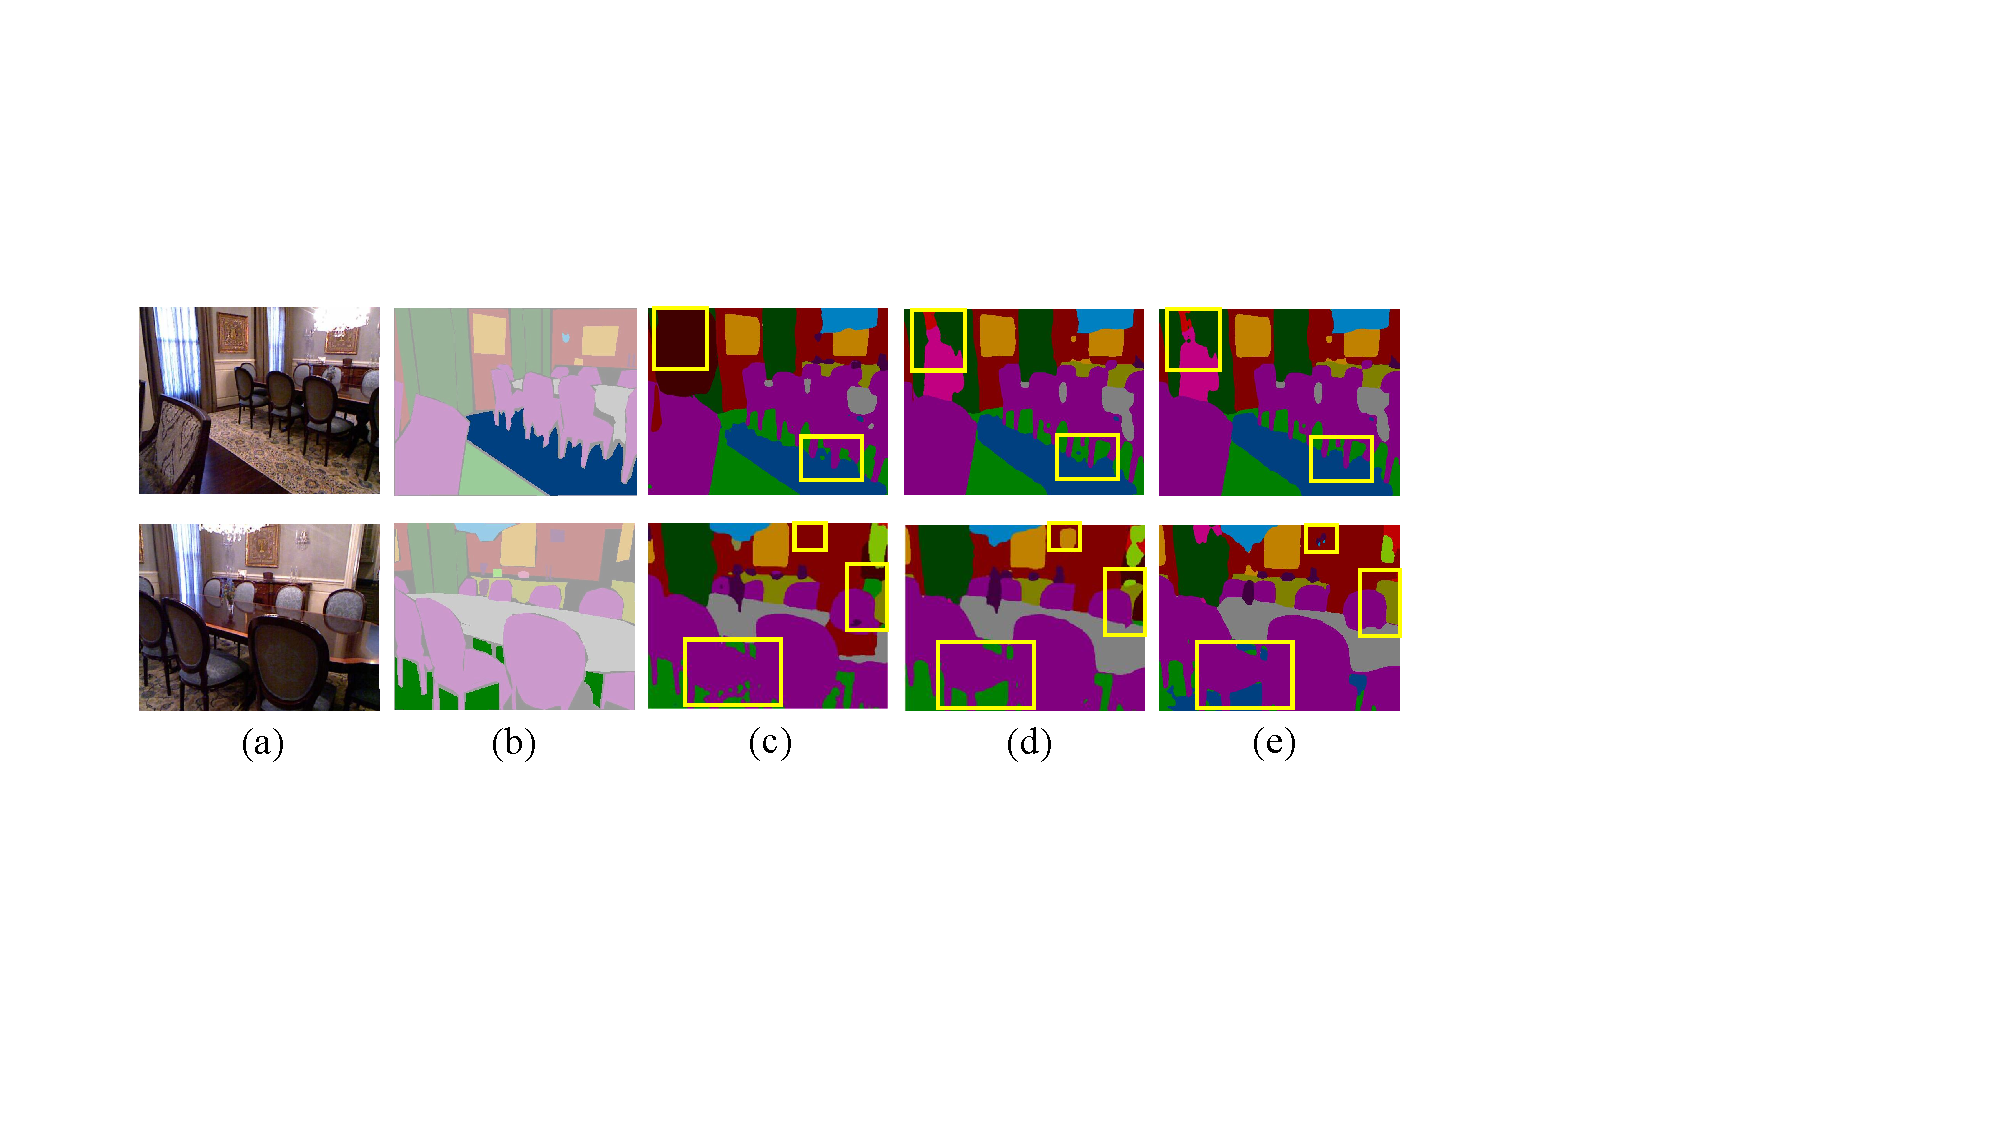
\includegraphics[scale=0.4]{figure/Mislabels.pdf}
	\caption{Mislabeled images. (a) Two frames of the same scene. (b) Their corresponding ground truth labels. Note the difference between the labels of the floor pixels. Blue as "floor mat" and green as "floor".  The mislabled pixels are highlighted. (c)(d)(e) The prediction results of RefineNet, RDFNet and our method, respectively.}
	\label{fig:mislabels}
\end{figure}
%

\begin{comment}{
But our proposed method shows a more robust result compared to RefineNet \cite{Lin2017} and RDFNet \cite{Park2017}.
%
}
\end{comment}






\section{Conclusion}
\label{sec:conclusion}
In this paper, we introduce two effective semi-supervised approaches for exploiting unlabeled frames in videos to improve semantic segmentation performance of indoor scenes. 
%In order to make full use of unlabeled samples, 
First, we propagate the labeled data to neighboring frames and generate a large number of reliable pseudo labels to enrich the training set.
%Despite the existence of noisy labels in PGT, the network can still learn more abundant information from PGT.
%
Second, our training policy takes advantage of temporal correlations between adjacent frames to enhance the semantic segmentation performance.
%
Experimental results on NYUD-v2 dataset demonstrate the superiority of our proposed method.  
%{\bf Future Work.} As we said in the discussion, the imbalance of sample classes results in the error of segmentation results. 
%
%Hence, our future work is still based on the data itself.
%
%One direction is how to balance sample categories, and the other is how to make more efficient and reasonable use of unlabeled video data.



\bibliographystyle{IEEEbib}
\bibliography{strings,refs}


\comments{
\begin{thebibliography}{00}
\bibitem{b1} G. Eason, B. Noble, and I. N. Sneddon, ``On certain integrals of Lipschitz-Hankel type involving products of Bessel functions,'' Phil. Trans. Roy. Soc. London, vol. A247, pp. 529--551, April 1955.
\bibitem{b2} J. Clerk Maxwell, A Treatise on Electricity and Magnetism, 3rd ed., vol. 2. Oxford: Clarendon, 1892, pp.68--73.
\bibitem{b3} I. S. Jacobs and C. P. Bean, ``Fine particles, thin films and exchange anisotropy,'' in Magnetism, vol. III, G. T. Rado and H. Suhl, Eds. New York: Academic, 1963, pp. 271--350.
\bibitem{b4} K. Elissa, ``Title of paper if known,'' unpublished.
\bibitem{b5} R. Nicole, ``Title of paper with only first word capitalized,'' J. Name Stand. Abbrev., in press.
\bibitem{b6} Y. Yorozu, M. Hirano, K. Oka, and Y. Tagawa, ``Electron spectroscopy studies on magneto-optical media and plastic substrate interface,'' IEEE Transl. J. Magn. Japan, vol. 2, pp. 740--741, August 1987 [Digests 9th Annual Conf. Magnetics Japan, p. 301, 1982].
\bibitem{b7} M. Young, The Technical Writer's Handbook. Mill Valley, CA: University Science, 1989.
\end{thebibliography}
}
\end{document}
